% #############################################################################
% This is Chapter 5
% !TEX root = ../main.tex
% #############################################################################
% Change the Name of the Chapter i the following line
\fancychapter{Implementation}
\cleardoublepage
% The following line allows to ref this chapter
\label{chap:implementation}

This chapter presents the details of the developed solution on the HSM, the user software and the developed API, which accesses the HSM services.
It covers the implementation details, namely the standards and libraries, the developed services, their logic and how the device's accelerators are leveraged. The main components are the communications, secure data exchange service, digital signatures, key management solution and tamper detection features.

% -----------------------------------------------------
\section{Libraries and Tools}\label{chap:implementation:tools}

The device's implementation is running on the SoC of a SmartFusion2 board, version M2S090TS from Microsemi, presented in Section \ref{chap:background:computing:smartfusion}.
The application was implemented using the C programming language, with the SoftConsole version 3.4 \ac{IDE} provided by Microsemi. The board was configured using Libero version 12.2.
The device functions as a HSM, connected through a serial connection to a computer. It was programmed using the external FlashPro4 programmer, required to develop and debug embedded applications with the SoftConsole IDE \cite{smartfusionSecurityPractices}.

A common developer interface, to access the device's services, was implemented using the PKCS\#11 standard, in order to standardize the accessibility of its services to other systems. The developed user application has a simple \ac{CLI} interface, which invokes the PKCS\#11 functions.
Both the software and the API were implemented in C/C++, for the open source MinGW compiler for Windows 10.
The device implementation uses the available \ac{UART} communication controller and corresponding drivers for communications, while the user application uses the windows drivers to communicate with serial ports.

% -----------------------------------------------------
\section{HSM Services}\label{chap:implementation:services}

The services were implemented using the SmartFusion2 security accelerators: SRAM-PUF, AES, HMAC, SHA, ECC, TRNG and tamper detection.
All the implemented services are accessed through the developed PKCS\#11 API, with the communication protocols detailed in Section \ref{chap:arch:services}.

By default, the device's RAM has 64 KB for running code. For each byte of the \ac{RAM}, there are 2 bits for error detection and correction, a total of 16 KB. This feature mitigates \ac{SEU}, which can flip memory bits. It corrects 1 bit errors and detects up to 2 bit errors. If more memory is needed for more application code, the board can be configured with this setting disabled in Libero. This frees the additional 16 KB of memory for RAM, for a total of 80 KB.
% The developed implementation configured the board with this feature off, in order to use 80 KB of RAM for code.

% -----------------------------------------------------
\subsection{Login}\label{chap:implementation:services:authentication}

Entities must be authenticated before they can access the device's services. The login operation authenticates the user, using an eight digit PIN.
There is only a single PIN to authenticate the entity. The individual users are not authenticated.
The PIN is stored in the secure storage of the internal device. The available secure storage and management solutions which can be used to store the number are discussed in a section ahead.
Once the user is authenticated, the PIN can be altered by changing the existing value.

\subsection{Secure Communications}\label{chap:implementation:services:secure}

The goal of this service is to provide authentication and confidentiality to the data being exchanged, between entities with these devices, using internal keys.
In order to provide these services, a protocol was previously defined in Section \ref{chap:arch:services:data-exchange}, which combines a symmetric encryption and authentication scheme. The algorithms are combined with an encrypt-then-MAC approach, meaning the plaintext is encrypted first, then authenticated.

The SmartFusion2 SoC supports the type of algorithms needed for this protocol.
For every encryption operation, a random 16 byte IV is generated, using the TRNG service.
For symmetric key authentication, the board supports HMAC with the SHA-256 hash function, which uses a 256 bit symmetric key, to generate a 256 bit code. As discussed in Section \ref{chap:background:crypto:mac}, it is a well-designed construction, even though it is not the most efficient.
For confidentiality, the board provides several AES symmetric encryption modes, with 128 bit and 256 bit keys. Among them, CBC and CTR are the most favourable options because of their security.

When choosing key sizes, and taking into account the limited storage capacity of the board, a smaller, but still secure, key size is preferred. The AES 128 bit and 256 bit services guarantee 128 and 256 bit security respectively. HMAC with SHA-256 provides 256 bit security, with 256 bit keys.
According to the NIST recommendations~\cite{nistRecommendations}, algorithms which guarantee both 128 and 256 bit security, are expected to be secure until 2031 and beyond. If storage is extremely limited, AES with 128 bit keys is a secure and adequate option. However, with 256 bit security, the system will have a longer life expectancy.

The key used for HMAC should be different from the one used in encryption, to ensure the best security practices, by not reusing the same key in different algorithms. So in practice, a key used for securing communications is split in two keys, one for encryption and one for authentication.

The board was configured with its maximum of RAM, 80 KB. With all the code needed for this implementation, a maximum of 36 KB is available for the plaintext and ciphertext buffers.
Initially, two buffers of 18 KB each were used, one for the input data and one for the output result. This was improved to a single 36 KB buffer, where the initial input is stored, as well as the result while it is computed.
Therefore, with this protocol implementation, the system is limited to securing 36 KB of plaintext.
In order to improve this, a continuous cipher and authentication implementation is needed. The data would not be received in full, but instead, the data would be divided in chunks, which are received by the device, computed and returned to the user, one after the other. However, the board is not capable of continuous operations using the provided AES and HMAC implementations.

To overcome this limitation, the characteristics of the AES CBC mode can be taken advantage of, as pictured in Figure \ref{fig:protocol:cbc-chunks}. 
\begin{figure}[h!]
	\centering
	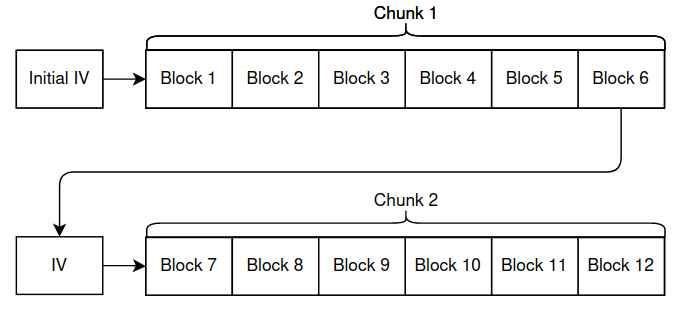
\includegraphics[width=0.75\textwidth]{./Images/cbc-chunks.png}
	\caption{Continuous CBC block encryption of data divided in chunks}
	\label{fig:protocol:cbc-chunks}
\end{figure}
CBC mode encrypts data one 16 byte block at a time, using an IV. The IV of the first block is the randomly generated value from the TRNG. The IV of the subsequent blocks, is the previously computed ciphertext block.
If the data is received in chunks, the IV of the first chunk is the randomly generated value, while the IV of the next chunks is the last ciphertext block of the previous chunk.
This allows continuous encryption of data divided in chunks.
For HMAC, a lightweight software implementation was included, to allow continuous authentication \cite{ogayHMAC}.

Since with this approach, the full data is divided in chunks, a modified communications protocol is necessary, so the device can receive and send the data, one chunk at a time.  The developed continuous communications protocol is depicted in Figure \ref{fig:protocol:data-exchange-chunks}.
\begin{figure}[h!]
	\centering
	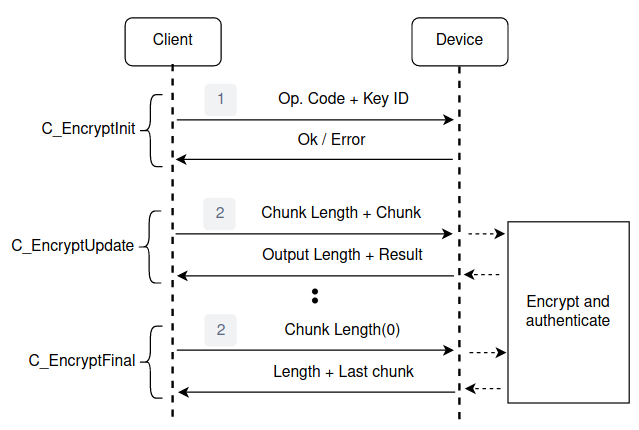
\includegraphics[width=0.75\textwidth]{./Images/data-exchange-chunks.png}
	\caption{Communication protocol for continuous data ciphering and authentication in the HSM with internal keys}
	\label{fig:protocol:data-exchange-chunks}
\end{figure}
The operation code identifying the service is sent first, along with the key ID which identifies the internal key stored in the device, with the initial call to the PKCS\#11 API.
Then, each subsequent call to the API, sends a chunk of data along with its length.
For each chunk received, the device adds the chunk to its buffer, encrypts the data, updates the HMAC calculation, and returns a ciphertext chunk.
When there are no more chunks to receive, the board returns the remaining ciphertext and final MAC value. The total output is composed of the initial IV, ciphertext and MAC.

The total data length is not sent initially, instead, the length of each chunk is sent before the chunk. This allows for a more flexible system. User applications calling the PKCS\#11 API, can send data to the device as it is needed, even if it does not have the complete data initially.
The downside of this approach is the device does not know the amount of data it will encrypt. The internal buffer must be managed, so it adds complexity to the implementation.

The reverse operation for authentication and decryption of data is exactly the same. The only change is the operation code value is different, so the device knows what operation to perform.
To avoid padding and guarantee CBC's security, ciphertext stealing was implemented.

As previously introduced, the board's AES implementation is not resistant to side-channel attacks, such as DPA. This means attackers with physical access to the device, can potentially read and compromise the keys stored internally. In order to mitigate this and build a more robust system, a 128 bit AES core implemented in the board's FPGA, resistant to side-channel attacks, was also tested with this service.

% -----------------
\subsection{Key Management}\label{chap:implementation:services:key-import}

Symmetric and asymmetric keys are essential for the functionality and security of the system and its services. Secure symmetric keys are necessary for the security of communications, while asymmetric keys are needed for key agreement and digital signatures.
All these keys are stored inside the device, and the system is responsible for their security and management. Thus, it is essential for the system to have a secure and flexible key management solution, which takes advantage of the device's secure storage.

As described in Section \ref{chap:background:computing:smartfusion}, the SmartFusion2 provides a secure storage service, the SRAM-PUF. It has 56 available key slots, where one key can be saved in each slot with a maximum of 512 bytes for a single key.
The service uses private eNVM blocks to store part of the key data. Since the eNVM is limited to 1000 writes for each page, for a predicted lifespan of 20 years. Thus, there is a limit on the key storage frequency in the slots. The service should be used carefully, restraining how often it is written to, in order to preserve its lifespan.

So as to mitigate the limitation of the PUF storage, an alternate solution, in which the keys are stored in a non volatile memory was developed, as depicted in Figure \ref{fig:implementation:key-management}.
\begin{figure}[h!]
	\centering
	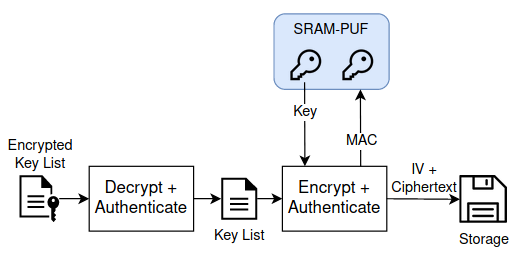
\includegraphics[width=0.45\textwidth]{./Images/key-management.png}
	\caption{Key management solution to store keys encrypted and authenticated in a non volatile memory using the SRAM-PUF secure storage}
	\label{fig:implementation:key-management}
\end{figure}
In order to securely store the keys, they must be encrypted so as to hide their contents, and authenticated to detect any unauthorized modifications.
To encrypt and authenticate keys, a symmetric key is necessary. This key is randomly generated in the device and stored in a dedicated PUF slot, only used for storing keys in memory.
The ciphertext of the keys is stored in memory, along with the IV used for encryption.
Both pieces of information are authenticated by generating a MAC, which is stored in another dedicated PUF slot.
With this solution, a key can be accessed by generating the MAC of the stored data and comparing it to the one stored in the PUF slot. If they match, the keys are authenticated, and can be decrypted with the IV and dedicated PUF key.

While this solution still uses the PUF service, its usage is more measured. When using the PUF service, when a key is stored one slot is written.
In the case of the implemented solution, for each change of the key list stored in memory, only the MAC slot is written to.
If keys are added one at a time, the amount of PUF slots written per key is identical for both options. However, multiple keys can be updated at once, if for example a list o f keys is imported. In this case, multiple keys can be added or updated, with only one write to a PUF slot.

The amount of available key storage is not a problem, since the board allows for external storage devices to be connected, where keys can be stored, encrypted and authenticated. If attackers get access to the key storage, the encrypted keys cannot be read, without the key protected in the SRAM-PUF.

This solution is design to store a list of keys. The service, introduced in Section \ref{chap:arch:services:new-comms:import}, for importation of keys was designed, in order to provide a list of keys for the key solution.
The service allows entities to receive a set of encrypted keys from another entity, forward the list to their device, which decrypts them with the secure data exchange service and stores them in the non volatile storage.
The entity from which the keys are received is responsible for the distribution of keys among entities. So as to communicate with the trusted entity, all devices are delivered with a stored symmetric key for secure communications with the entity.

% -----------------
\subsection{Key Generation}\label{chap:implementation:services:key-generation}

The goal of this service is to enable agreement of symmetric keys between entities with these devices. This enables entities with no previously agreed keys, to securely communicate with each other using the devices.
This service takes advantage of public-key cryptography in order to agree on a key.
The key generation service follows the protocol and guidelines defined in the previous Section \ref{chap:arch:services:new-comms:ecdh}.
Both entities have a private and public key pair. After sharing public keys with each other, they can generate the same secret using their private key and the public key of the other entity.
The SmartFusion2 SoC provides the necessary ECC scalar multiplication accelerator, to generate a shared key with the ECDH algorithm. The accelerator multiplies the 48 byte private key with a 96 byte public key to generate a 96 byte shared value, which can be stored using the system's key management solution.

% -----------------
\subsection{TCP Channel}\label{chap:implementation:services:secure:tcp}

With the secure data exchange service, entities can securely trade messages using an offline service such as e-mail or an online chat service.
In order to truly establish a secure communication channel, and demonstrate the common developer interface, the secure data service was used to encrypt and authenticate a TCP connection. A TCP implementation using Windows sockets is used to exchange data through a channel, between a client and server, running on the same computer. As pictured in Figure \ref{fig:implementation:tcp}, the library was altered, to call the PKCS\#11 API of the SmartFusion2 system, to encrypt the plaintext data in each TCP packet, before it is sent. Likewise, when a packet is received, the decryption API is called, in order to retrieve the plaintext.
\begin{figure}[h!]
	\centering
	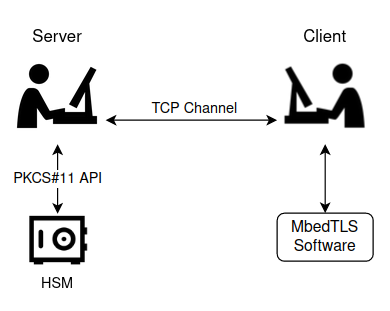
\includegraphics[width=0.5\textwidth]{./Images/tcp.png}
	\caption{TCP connection between a server using the HSM system through PKCS\#11 API calls and a client running a MbedTLS implementation}
	\label{fig:implementation:tcp}
\end{figure}
Before a secure TCP connection is established, both entities must agree on a symmetric session key, which will be used to encrypt and authenticate the connection. This is achieved by using the previously described key generation service with ECDH. After each side trades their public keys on the P-384 curve, they can compute the same symmetric key. In order to emulate two communicating entities using a similar system, one side is running a local implementation of the same cryptographic services of the proposed system, with the mbedTLS 2.26.0 library.

% -----------------
\subsection{Qualified Digital Signatures}\label{chap:implementation:services:signatures}

The goal of digital signatures is to provide non-repudiation to messages. This prevents an entity from denying the authorship of a message. 
The service was designed to provide an improved version of signatures, called qualified digital signatures, where the private keys, which generate signatures, are stored inside the HSM, and are never exposed to the outside.
This guarantees the signature generator is someone with access to the device holding the private key.

The SmartFusion2 SoC provides ECC key support which can be used to generate signatures with the ECDSA algorithm. However, the board does not provide an ECDSA implementation. Either the board uses an external source for digital signature generation, which would cease to be qualified, or the algorithm is implemented in the board.

In general, the ECDSA algorithm is composed of two types of operations. ECC operations, e.g., scalar multiplication and point addition, which are supported by the board. The other is large numbers arithmetic operations, such as, modular multiplications and divisions. These operations are not supported by the board, a big numbers library is necessary. In case of the supported P-384 curve, the library should support operations between 48 byte numbers. 

Thus, a big numbers library was included in the system \cite{libecc}. The library was stripped of all unnecessary code and headers, keeping the necessary big integer operations. The ECC primitives and true random number generator were included in the library code. Digital signature generation was implemented, without verification. The library takes up around 54 KB of RAM space. Thus, this functionality only works with a limited buffer size of around 1.5 KB, if all other implemented services are disabled.
This is an extremely limited use case, and less than ideal. Future work should revise this functionality, by evaluating existing lightweight libraries, which provide the necessary features, or even a custom implementation.

% -----------------
\subsection{Tamper Detection}\label{chap:implementation:services:tamper-detection}

An important part of a HSM based system is physical protections against tampering and attacks.
In order to defend the system against physical threats, the tamper detection, zeroization and secure boot functionalities of the SmartFusion2 SoC were taken advantage of.

Tamper attacks and possible attempts can be detected by the board. When these events occur, flags are asynchronously set, which warn the user from potential anomalies, errors and attacks. With this information, measures, such as zeroization, can be taken to protect the system.
Zeroization is a process which erases all sensitive information from the device. This process can place the device in three possible states. It can be rendered permanently unusable, reset to its initial state or recoverable only with a key file supplied by Microsemi.

Another security measure of the SmartFusion2 board, is the computation of digests from the eNVM blocks and fabric configuration, which also holds the code. Every time the board is programmed or the configuration is changed, new digests are computed and stored in secure storage. On boot, the board computes the digests and compares them to the stored values. This allows the board to safeguard the integrity of its storage and configuration.

When the tamper attacks are flagged in the implemented system, the device does not accept any more PKCS\#11 calls and zeroization is performed on the device, erasing all keys, configuration and data. Additionally, the secure boot checks are turned on.
Zeroization was configured to reset the device to its initial state from fabric.
The user also has the option to manually trigger zeroization, by pressing a switch on the board.
These measures can have a denial-of-service effect on the system, but are a trade-off deemed necessary, in order to avoid successful attacks and potential leaks of sensitive information.

% -----------------------------------------------------
\section{PKCS\#11 API}\label{chap:implementation:app:pkcs}

In order to demonstrate the flexibility of the system, a PKCS\#11 API was developed to access the HSM services. Developers who wish to use this system for future work on a SmartFusion2 SoC, can call this API from the developed software.
The PKCS\#11 implementation supports one token with one session.
PKCS\#11 defines two types of users, the regular user and the security officer. The implementation does not make that distinction. Both types of user can login, and gain access to all other services.
The full list of the implemented PKCS\#11 functions, their arguments and description are listed in Table \ref{tab:pkcs11-api}.

% -----------------------------------------------------
% -----------------------------------------------------
\section*{Summary}\label{chap:implementation:summary}

This chapter presented a proof of concept implementation of a HSM application supported on a SmartFusion2 device, using its security services and accelerators. It specified the used libraries and tools, all implemented services motivation, details, advantages and drawbacks, as well as the developed PKCS\#11 API to access these services. The prototype focused on secure communications with authentication and confidentiality. It provided improvements on the architecture baseline set in Chapter \ref{chap:arch}, using the device's capabilities and benefiting from some software implementations. It also provided flexibility with a key management solution, using the board's secure storage efficiently, new key generation and qualified digital signatures using public-key cryptography features.
The work also explored the device's drawbacks and provided possible ways to mitigate them. Lastly, it presented the available tamper detection options and zeroization features, with implementation examples.
